\chapter{Initial Testing Results}
\label{sec: it1design}


% To see the design and results of iteration 1 please refer to Appendix \ref{sec: it1design}. 

\section{Iteration 1 Testing Results}
\label{subsec: it1results}
% Table \ref{tab:iter1results} shows the overview of the results from the acquired data from the feedback form from Iteration 1, while Table \ref{tab:iter2results} shows the results from Iteration 2. As mentioned, the feedback forms from those iterations differed, so the results and treatment of the data will be discussed separately in the following subsections.

\begin{table}[H]
\centering
\begin{tabular}{|l|l|l|l|l|l|l|} 
\hline
   & Age & Years & Sex & Hand & Instrument                                                          & Technique  \\ 
\hline
P1 & 8   & 1     & M   & R    & Drums                                                               & T          \\ 
\hline
P2 & 7   & 1     & F   & L    & \begin{tabular}[c]{@{}l@{}}Piano and \\Drums \end{tabular}          & T          \\ 
\hline
P3 & 5   & 1     & M   & R    & \begin{tabular}[c]{@{}l@{}}Piano, Guitar, \\and Drums \end{tabular} & T          \\
\hline
\end{tabular}
\caption{Participant Demographic. T - Traditional, S - Suzuki}
\label{tab:participant}
\end{table}


For the results of the first iteration of testing, first we processed the timestamps in order to normalize these values. This is important so we can properly understand the actual time it took them to finish the task, this can be seen in Figures \ref{fig:P1Timing}, \ref{fig:P2Timing}, and \ref{fig:P3Timing}. We then observed that due to other circumstances during the testing like the long duration and fatigue from school, in answering the questions the children sometimes mistook the scales in grading for the difficulty of the tasks. In some tasks they graded it much easier or harder than what we observed as when we double checked and asked them to name the functionality of a specific part, they were mixing up some of the functionality yet still for example give a score of (1) where they fully remembered it. Due to this their initial scores were then cross referenced to the task they were given and if we observed that there was a big difference in the answer and our observation an adjustment of  + 1 or - 1 was changed in the scores to balance these out. 

The red bar indicates the level of difficulty that the user has chosen for the task. The blue bar indicates the time for their time of completion for the task. To enhance the visualization we scaled the difficulty of 1-4 by multiplying it by 5 and divided their time by 5 so their correlation can be seen more in the graphs.

\begin{figure}[H]
    \centering
    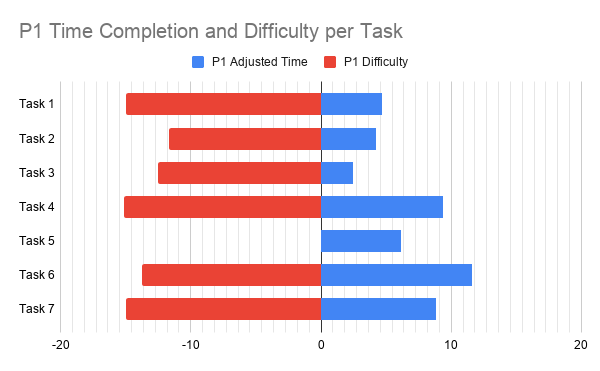
\includegraphics[width=8cm]{figures/NewFigures/P1.png}
    \caption{Time for Completion and Difficulty of Tasks for Person 1}
    \label{fig:P1Timing}
\end{figure}
 P1 (8, M, Drums) believes that task 4, which was the tail, was most likely not intuitive for him to change because it took him a longer time and he rated it as a higher difficulty compared to playing with the other body parts. Task 6 and 7 took a long time because it was mostly playing around with the application.
 
\begin{figure}[H]
    \centering
    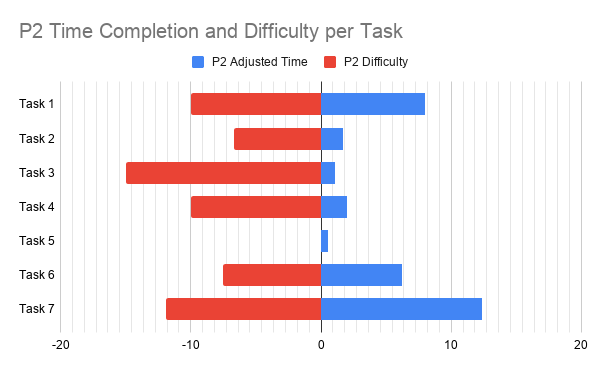
\includegraphics[width=8cm]{figures/NewFigures/P2.png}
    \caption{Time for Completion and Difficulty of Tasks for Person 2}
    \label{fig:P2Timing}
\end{figure}
P2 (7, F, Piano) believes that task 2, which is the body, was most likely not intuitive because it took her a long time to complete. It can also be seen also that she did not grade the difficulty as high as person 1 because she has more experience in music.

\begin{figure}[H]
    \centering
    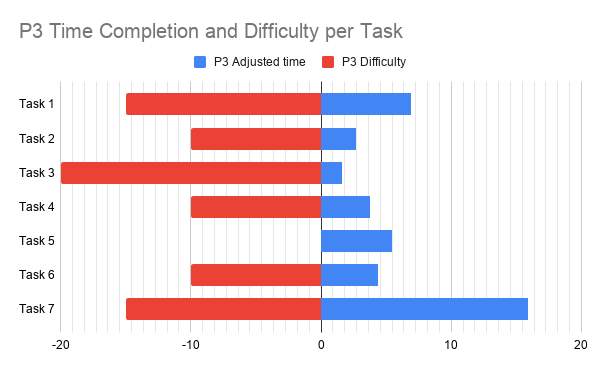
\includegraphics[width=8cm]{figures/NewFigures/P3.png}
    \caption{Time for Completion and Difficulty of Tasks for Person 3}
    \label{fig:P3Timing}
\end{figure}
P3 (5, M, Guitar) similar to P2 took a lot of time in performing task 1 which supports that it most likely not intuitive.


% Based on observations and comments from the Focus Group Discussions, participants appreciated and had a more positive response to the louder and faster songs. All participants agreed that the inclusion of speakers for haptic feedback and colors would improve their experience, as such this was considered for the Iteration 2 experiments. The participants were easily bored due to the grayscale color scheme of the prototype. The participants provided more recommendations such as (1) adding the lyrics as captions (2) visuals of the singer singing the song and (3) adding more visual elements.

% Based on the data in Figure \ref{tab:iter1results}, we computed for the correlation coefficients of BPM with average score and BPM with standard deviation, which can be seen in Table \ref{tab:correlations}. Based on these statistical figures, BPM and average score, as well as standard deviation have no correlation.
% %The computed correlation coefficient for BPM and average score is 0.1294, which is interpreted as little positive correlation. The computed correlation coefficient for BPM and standard deviation is 0.1145, which is also interpreted as little correlation.

% Despite the explicit statements from the participants that they appreciated the louder and faster songs, analysis of the statistical results show that their scores were not consistent. Faster and louder songs did not necessarily have the higher ratings. This may be attributed to mismatches regarding visual impact. The songs may not have had their musical features represented consistently and fairly enough for them to appreciate the experience.


\begin{figure}[H]
    \centering
    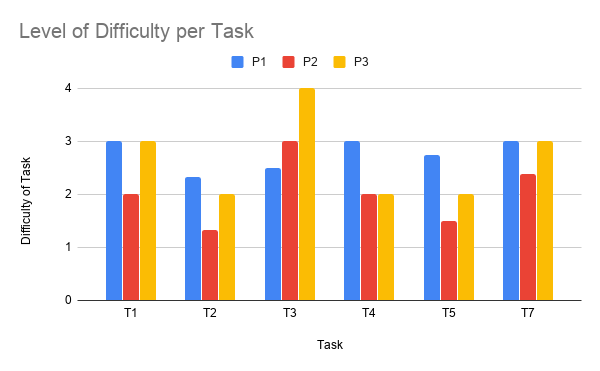
\includegraphics[width=8cm]{figures/NewFigures/DifficultyTask.png}
    \caption{Difficulty of Tasks for each User}
    \label{fig:DifficultyofTask}
\end{figure}
\begin{figure}[H]
    \centering
    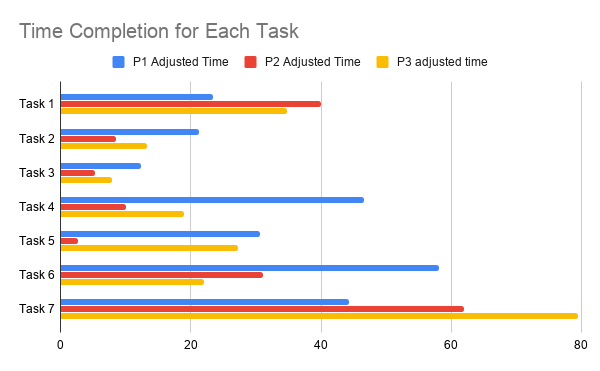
\includegraphics[width=8cm]{figures/NewFigures/AllTime.png}
    \caption{Time Completion of Tasks for each User}
    \label{fig:TimeofTask}
\end{figure}

\subsection{Participant Insights}

\begin{figure}[H]
    \centering
    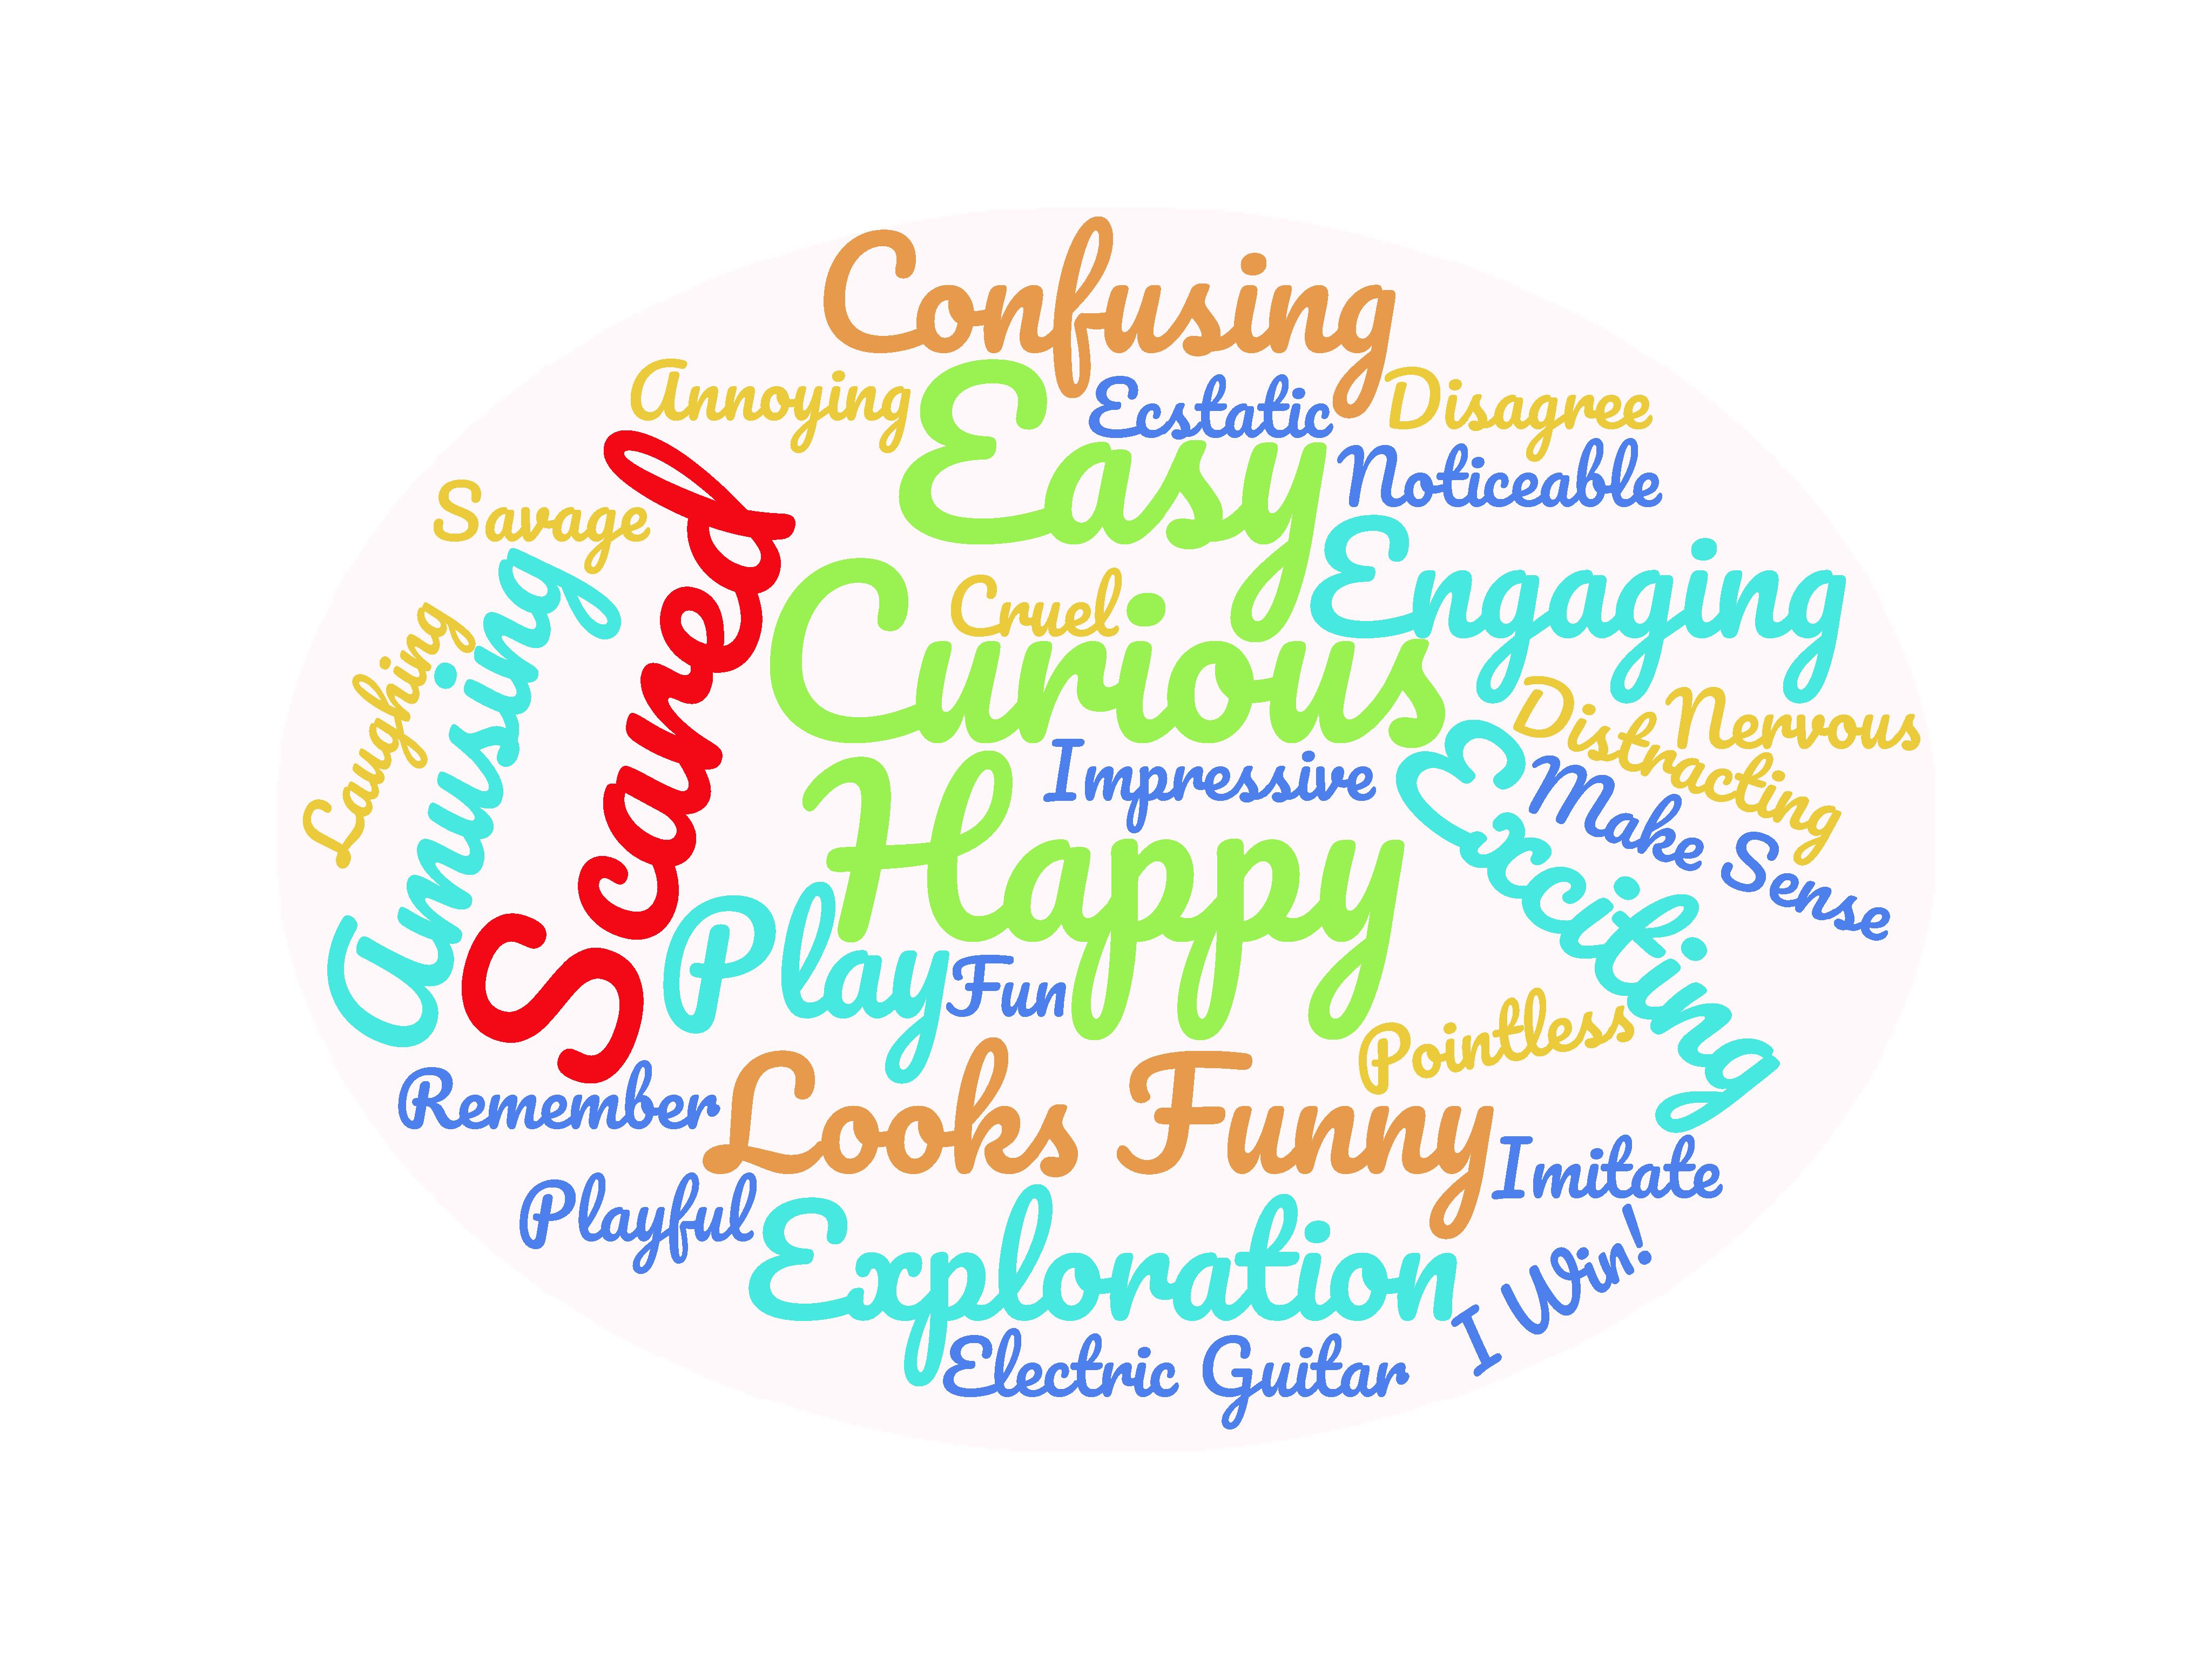
\includegraphics[width=9.5cm]{figures/NewFigures/wordcloud.jpg}
    \caption{Word Cloud of Positive and Negative Comments}
    \label{fig:wordcloud}
\end{figure}

% \begin{figure}[H]
%     \centering
%     \includegraphics[width=8cm]{NewFigures/negativeWordcloud.jpg}
%     \caption{Word Cloud of Negative Comments}
%     \label{fig:negative}
% \end{figure}


\section{Discussion}

It can be seen clearer in Section 4.5 that majority of them took longer in playing with the body part, which is task 1. And upon further observation one of the underlying reasons could be that they tend to miss the hotspot for pressing the body part.  We also noticed that most of them would pick their favorite color for the body part, which they enjoyed. It can also be seen that Task 3 which is changing the size of the wings for repetition took them the fastest time to complete

Based on our user testing for iteration one, as seen in Figure \ref{fig:DifficultyofTask}, task two, which was to change the speed of the first note using the left wing, took the shortest time to complete and had the lowest difficulty for the users. However, in task two only two out of three users noticed the lever for changing the note to rest or beat. Then task 3, which was to change the number of repetitions by tapping the right wing, took the longest time and had the highest difficulty for the users. We also observed that all participants use their dominant hand most of the time when using the application as P1 and P3 were both right handed as P2 was the only one that was left handed. During the interview some had a hard time remembering which part of the firefly changed each property when they were asked which part did what. The one with most music experience mentioned that the app didn't help much in retaining her music lessons, and then suggested that we utilize a music staff. We observed their behavior when using the application and we noticed that they were eager to explore features that they think is clickable even when the tasks were not yet given to them. We also noticed that in features like the lever, they would use a flick gesture imitating how it is usually used instead of the tap gesture that we set it to be. 

 As seen in Figure \ref{fig:wordcloud} during testing while they were doing their tasks we took note of their comments and interpreted them in a general way or in terms of a feature that they commented on. The positive comments were represented using cool colors like blue and green, while negative comments were represented with warm colors like red and orange. For the positive comments we observed that aside from us noticing their curiosity in using the application, they themselves say that they are curious when doing their tasks. We can also see that they have comments about being playful and having fun while using the application. In terms of the interface, comments like "Make Sense" and "Engaging" indicated to us that there are features that they like and that some parts of the interface is good for them. For the negative comments, one comment that stood out to us was P3 mentioned that the animations of the firefly was "glitchy", this comment made us improve the assets for the animation for the next animation. The other negative comments like "Looks Funny" and "Distracting" indicated to us that there were some features that they wanted us to change in the interface. Lastly, even if the purpose of the sandbox environment was for the users to play without breaking anything, P3 still said he was "Scared" multiple times to ruin the firefly and we think that this has to do with his young age and also for us to put information on the screen so that the children will not be discouraged to play with the firefly.